\section{Final testing and conclusions}\label{sec:conclusions}

Once we refined our model at the best could, we evaluated it against never seen data, by comparing the values predicted by the model, when the testing set is provided as input, against the true values of the annotations in the testing set. As already mentioned in section~\ref{sec:cross-validation}, once the final testing is done, we avoided going back to the model and make further tweaks, as this would have led to over-fitting.

For the final test we used the metrics of MSE and $R^2$-score (see section~\ref{sec:metrics}) and obtained the values reported in table~\ref{table:eval-metrics}. By comparing these values with the ones of table~\ref{table:cross-scores}, it can be noticed that they are very similar and within the ranges provided by the cross-validation. This demonstrates the usefulness of this type of operation and the fact that our model is quite robust.
 \todo[inline]{ultima frase boh, si puuuò anche togliere}


We also extracted scatter plots comparing the predictions of each regressor against the true values of the testing set. In  figure~\ref{fig:eval-scatter} is depicted the case of $\nu$-SVM, which turned out to be the best model fitting the data. In the best case scenario, these scatters should draw a 45° line. In our case, the scattering of ``valence std'' and ``arousal std'' clearly outline the bad $R^2$-scores obtained for these annotations.

As mentioned before a possible motivation for our results could be related to the composition of the dataset and the fact that we used only the part containing static annotations. A possible way to continue this researh could be to adopt a dynamic approach in which we consider values related to temporal windows instead of to the total length of the music piece as we have done in the study described in this paper. 


\begin{table}
	\centering
	\subcaptionbox{MSEs}{
		\begin{tabular}{lcccc}
			\toprule
			& valence mean & valence std & arousal mean & arousal std \\
			\midrule
			Ridge & 0.53 & 1.09 & 0.54 & 1.18 \\
			$\nu$-SVM & 0.58 & 1.00 & 0.49 & 1.09 \\
			K-neighbors & 0.62 & 1.00 & 0.61 & 1.08 \\
			\bottomrule
		\end{tabular}
	}
	\subcaptionbox{$R^2$-scores}{
		\begin{tabular}{lcccc}
			\toprule
			& valence mean & valence std & arousal mean & arousal std \\
			\midrule
			Ridge & 0.45 & -0.08 & 0.45 & -0.09 \\
			$\nu$-SVM & 0.40 & 0.01 & 0.50 & 0.00 \\
			K-neighbors & 0.35 & 0.01 & 0.39 & 0.00 \\
			\bottomrule
		\end{tabular}
	}
	\caption{Final evaluation metrics}
	\label{table:eval-metrics}
\end{table}

\begin{figure}
	\centering
	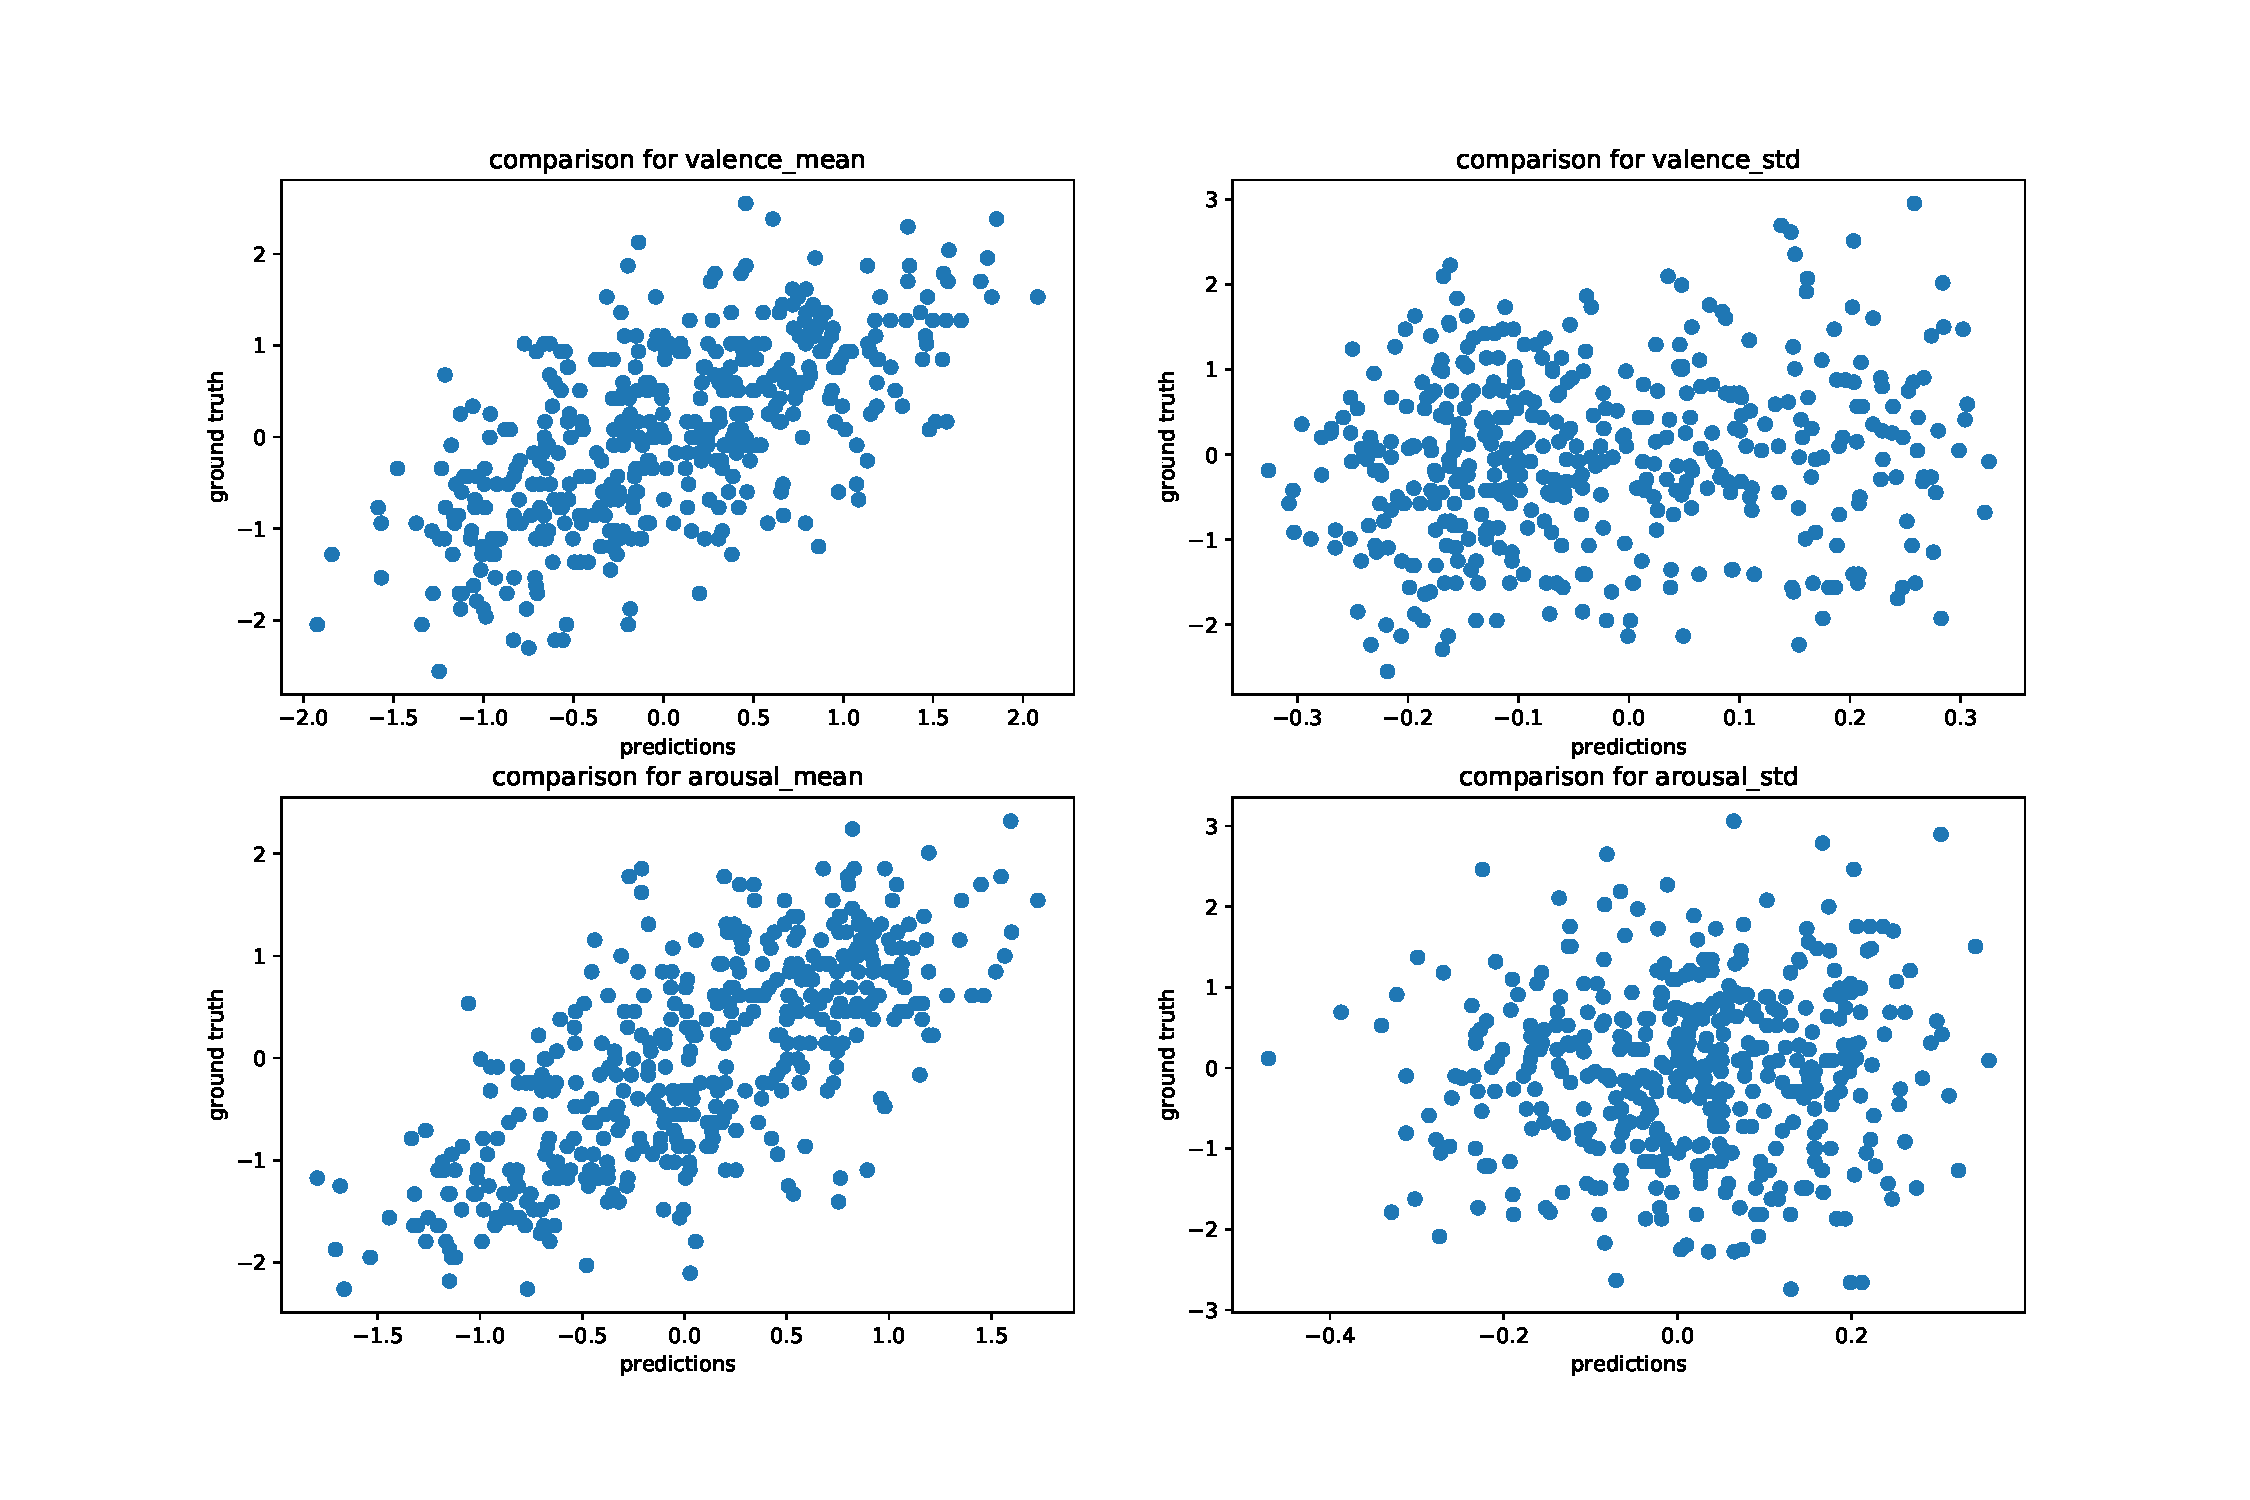
\includegraphics[width=\linewidth]{assets/predictions-scatter.pdf}
	\caption{predictions vs. ground-truth scatter for SVM regression}
	\label{fig:eval-scatter}
\end{figure}


